\upaper{43}{СОЗВЕЗДИЯ}
\uminitoc{СТОЛИЦА СОЗВЕЗДИЯ}
\uminitoc{ПРАВИТЕЛЬСТВО СОЗВЕЗДИЯ}
\uminitoc{ВСЕВЫШНИЕ НОРЛАТИАДЕКА}
\uminitoc{ГОРА СОБРАНИЯ~--- ОТ ВЕКА ВЕРНЫЙ}
\uminitoc{ОТЦЫ ЭДЕНЦИИ СО ВРЕМЕНИ ВОССТАНИЯ ЛЮЦИФЕРА}
\uminitoc{САДЫ БОГА}
\uminitoc{УНИВИТАЦИИ}
\uminitoc{УЧЕБНЫЕ МИРЫ ЭДЕНЦИИ}
\uminitoc{ГРАЖДАНСТВО НА ЭДЕНЦИИ}
\author{Малаватия Мелхиседек}
\vs p043 0:1 Урантию обычно называют 606-й Сатании в Норлатиадеке Небадона, что означает 606-й обитаемый мир в локальной системе Сатания, расположенной в созвездии Норлатиадек, одном из 100-а созвездий локальной вселенной Небадон. Так как созвездия являются первичными подразделениями локальной вселенной, их правители связывают локальные системы обитаемых миров с центральной администрацией локальной вселенной на Спасограде, а с помощью системы отражения со сверхадминистрацией От Века Древних на Уверсе.
\vs p043 0:2 \pc Правительство вашего созвездия расположено в скоплении из 771-й архитектурной сферы, центральной и крупнейшей из которых является Эденция~--- резиденция администрации Отцов Созвездия, Всевышних Норлатиадека. Сама Эденция приблизительно в 100 раз больше вашего мира. 70 больших сфер, окружающих Эденцию, примерно в 10 раз превышают размер Урантии, в то время как 10 спутников, которые вращаются вокруг каждого из этих 70-и миров, размером почти с Урантию\fnst{Обратите внимание, что эти пропорции справедливы и для архитектурных сфер локальной системы (см.\,\bibref[45:0.1]{p045 0:1}). Предполагая, что они остаются верными для скопления сфер Спасограда, мы можем вычислить общую площадь поверхности всех архитектурных миров (сравни с примечанием \bibref[37:10.1]{p037 10:1}): $10^4 + 70*10^2 + 70*6 + 100*(10^4 + 70*10^2 + 70*10) + 10\,000*(10^4 + 7*10^2 + 7*7) = 109\,277\,420$. Это более чем в 10 раз больше, общей поверхности всех эволюционных миров.}. Эти 771-а архитектурные сферы вполне сопоставимы по размеру с аналогичными сферами других созвездий.\tunemarkup{pictures}{\begin{figure}[H]\centering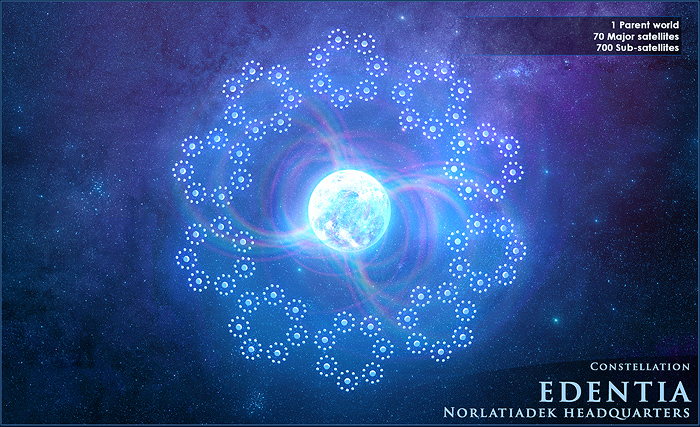
\includegraphics[width=0.98\columnwidth]{images/EDENTIA-700.jpg}\caption{Эденция от Гари Тонга}\end{figure}}
\vs p043 0:3 \pc На Эденции принята система исчисления времени и измерения расстояний Спасограда и, подобно сферам вселенской столицы, столичные миры созвездия полностью обеспечены всеми категориями небесных разумных существ. В целом, эти личности мало чем отличаются от тех, что описаны в связи с управлением вселенной.
\vs p043 0:4 Надзирающие серафимы, третья категория ангелов локальной вселенной, назначаются на службу в созвездия. Они располагают свои центры на столичных сферах и активно служат окружающим мирам моронтийного обучения. 70 больших сфер Норлатиадека, вместе с 700-ми малыми спутниками, населены унивитациями~--- постоянными гражданами созвездия. Все эти архитектурные миры полностью управляются различными группами местной жизни, по большей части нераскрытыми, но в число которых входят эффективные спиронги и прекрасные спорнагии. Моронтийная жизнь созвездий, являясь средней точкой в процессе моронтийной подготовки, одновременно и типична, и идеальна, как это и следовало ожидать.
\usection{СТОЛИЦА СОЗВЕЗДИЯ}
\vs p043 1:1 Эденция изобилует очаровательный нагорьями, обширными возвышенностями из физической материи, увенчанными моронтийной жизнью и преисполненными духовного великолепия, но там нет тех крутых горных хребтов, что встречаются на Урантии. Там есть десятки тысяч искрящихся озёр, и многие тысячи соединяющихся друг с другом ручьёв, но нет ни огромных океанов, ни стремительных рек. Только нагорья свободны от этих поверхностных потоков.
\vs p043 1:2 Вода Эденции и похожих архитектурных сфер ничем не отличается от воды эволюционных планет. Водные системы таких сфер бывают как поверхностными, так и грунтовыми, а влага находится в постоянной циркуляции. По этим различным водным маршрутам можно обогнуть всю Эденцию, однако основной транспортной средой является атмосфера. Духовные существа естественным образом путешествуют над поверхностью сферы, в то время как моронтийные и материальные существа для преодоления атмосферы используют материальные и полуматериальные средства передвижения.
\vs p043 1:3 Эденция и связанные с ней миры обладают настоящей атмосферой, обычной смесью трёх газов, которая характерна для таких архитектурных творений и включает два элемента атмосферы Урантии плюс моронтийный газ, пригодный для дыхания моронтийных созданий. Но хотя эта атмосфера и материальна, и моронтийна, штормов и ураганов там не бывает; не бывает также ни лета, ни зимы. Это отсутствие атмосферных возмущений и сезонных колебаний позволяет украсить всё внешнее пространство на этих специально созданных мирах.
\vs p043 1:4 Физические особенности нагорий Эденции великолепны, и их красота усиливается бесконечным богатством жизни, изобилующей на всём их протяжении. За исключением нескольких довольно изолированных строений, эти нагорья не содержат ничего рукотворного. Материальные и моронтийные украшения ограничены жилыми районами. Меньшие возвышенности~--- это места расположения особых резиденций и предстают в изысканной красоте как биологического, так и моронтийного искусства.
\vs p043 1:5 \pc На вершине седьмой гряды нагорий расположены залы воскрешения Эденции, где пробуждаются восходящие смертные вторичного модифицированного порядка восхождения. Эти палаты восстановления созданий находятся под наблюдением Мелхиседеков. Первая из принимающих сфер Эденции (подобно планете Мелхиседек возле Спасограда) также имеет специальные залы воскрешения, где восстанавливаются смертные модифицированных порядков восхождения.
\vs p043 1:6 Мелхиседеки также содержат на Эденции два специальных колледжа. Один из них, школа чрезвычайных ситуаций, занимается изучением проблем, возникших в результате восстания в Сатании. Другой, школа посвящения, предназначается для досконального изучения новых проблем, связанных с завершающим посвящением Михаила на одном из миров Норлатиадека. Этот последний колледж был учреждён почти 40\,000\fnst{В тексте 1955 года было указано <<четыре тысячи>>. Исправление во втором издании кажется оправданным на основании ссылки \bibref[119:7.2]{p119 7:2} в тексте: <<Публичное объявление о том, что Михаил выбрал Урантию в качестве театра для своего последнего посвящения, было сделано вскоре после того, как мы узнали о невыполнении обязательств Адамом и Евой. Таким образом, на протяжении более тридцати пяти тысяч лет ваш мир занимал очень видное место в советах всей вселенной. Проступок был совершён около 37\,800 лет назад, поэтому <<почти сорок тысяч>> и <<более тридцати пяти тысяч>> кажутся одинаково разумными описаниями. Комитет пришёл к выводу, что проблема по происхождению здесь идентична проблеме \bibref[41:4.4]{p041 4:4} в тексте: рассматриваемое число было написано в рукописи как цифра (40\,000, а не сорок тысяч), а ошибка была вызвана потерей нуля до того, как число было отформатировано в слова для печати.} лет назад непосредственно после провозглашения Михаилом, что Урантия выбрана в качестве мира его завершающего посвящения.
\vs p043 1:7 \pc Стеклянное море, принимающая область Эденции, находится недалеко от административного центра и окружено столичным амфитеатром. Вокруг этой области находятся управляющие центры 70-и подразделений, относящихся к делам созвездия. Половина Эденции разделена на 70 треугольных секций, границы которых сходятся в зданиях центров соответствующих секторов. Остальная часть этой сферы представляет собой один огромный природный парк~--- сады Бога.
\vs p043 1:8 Хотя во время периодических посещений Эденции твоему взору будет открыта вся планета, б\'ольшую часть времени ты будешь проводить в административном треугольнике, номер которого соответствует номеру мира твоего текущего пребывания. Ты всегда будешь радушно принят в законодательных ассамблеях в качестве наблюдателя.
\vs p043 1:9 Моронтийная область, отведённая постоянно проживающим на Эденции восходящим смертным, находится в средней области 35-го треугольника, который примыкает к центру завершителей, расположенному в 36-м треугольнике. Главный центр унивитаций занимает огромную область в средней части 34-го треугольника, непосредственно примыкающего к месту, отведённому для проживания моронтийных граждан. Как видно из этой планировки, предусмотрено размещение как минимум 70-и основных разделов небесной жизни, причём каждая из этих 70-и треугольных областей соотносится с какой\hyp{}либо из 70-и основных сфер моронтийной подготовки.
\vs p043 1:10 Стеклянное море Эденции представляет собой один огромный круглый кристалл примерно 160\,км в окружности и около 48\,км в глубину. Этот великолепный кристалл служит в качестве принимающего поля для всех транспортных серафимов и других существ, прибывающих из-за пределов сферы; такое стеклянное море значительно облегчает посадку транспортных серафимов.
\vs p043 1:11 Кристаллическое поле подобное этому встречается почти на всех архитектурных мирах; и кроме своей декоративной ценности, оно служит многим целям, так как используется для представления сверхвселенской системы отражения собирающимся здесь группам и как фактор в технике преобразования энергии для изменения потоков пространства и для адаптации других поступающих потоков физической энергии.
\usection{ПРАВИТЕЛЬСТВО СОЗВЕЗДИЯ}
\vs p043 2:1 Созвездия~--- это автономные единицы локальной вселенной, каждое созвездие управляется в соответствии со своими собственными законодательными актами. Когда суды Небадона выносят решения по вселенским делам, все внутренние вопросы решаются в согласии с законами, действующими в соответствующем созвездии. Эти судебные постановления Спасограда вместе с законодательными актами созвездий исполняются администраторами локальных систем.
\vs p043 2:2 Таким образом, созвездия функционируют как законодательные или законотворческие единицы, в то время как локальные системы служат как исполнительные единицы, проводящие законы в жизнь. Правительство Спасограда является высшим судебным и координирующим органом власти.
\vs p043 2:3 \pc В то время как верховная судебная функция возложена на центральную администрацию локальной вселенной, в столице каждого созвездия существует два вспомогательных, но важных суда: совет Мелхиседеков и суд Всевышнего.
\vs p043 2:4 Все судебные проблемы сначала рассматриваются советом Мелхиседеков. Двенадцать представителей этой категории, получившие определённый необходимый опыт на эволюционных планетах и на столичных мирах систем уполномочены рассматривать улики, анализировать заявления и выносить предварительные вердикты, которые передаются в суд Всевышнего~--- правящего Отца Созвездия. Отделение смертных этого последнего суда состоит из семи судей, каждый из которых~--- восходящий смертный. Чем выше ты восходишь во вселенной, тем больше вероятность того, что ты будешь судим себе подобными.
\vs p043 2:5 \pc Законодательный орган созвездия разделён на три группы. Законодательная программа созвездия берёт начало в нижней палате восходящих, группе, возглавляемой завершителем и состоящей из 1000 смертных представителей. Каждая система для участия в этой совещательной ассамблее выдвигает по 10 представителей. На Эденции в настоящее время этот орган укомплектован не полностью.
\vs p043 2:6 Средняя палата законодателей составлена из серафических воинств и их партнёров, других детей Материнского Духа локальной вселенной. Эта группа насчитывает 100 членов и назначается надзирающими личностями, которые возглавляют различные виды деятельности, осуществляемые этими существами в созвездии.
\vs p043 2:7 Совещательный или высший орган законодателей созвездия состоит из палаты пэров~--- палаты божественных Сынов. Этот корпус избирается Всевышними Отцами и насчитывает 10 членов. Только Сыны с особым опытом могут служить в этой верхней палате. Эта расследующая факты и экономящая время группа очень эффективно служит обоим низшим подразделениям законодательной ассамблеи.
\vs p043 2:8 Объединённый совет законодателей состоит из трёх членов от каждой из этих отдельных ветвей совещательной ассамблеи созвездия и возглавляется правящим младшим Всевышним. Эта группа утверждает окончательную форму всех законодательных актов и санкционирует их обнародование посредством трансляций. Утверждение этой верховной комиссией делает законодательные акты законом данной области; их постановления являются окончательными. Законодательные заключения Эденции составляют основной закон для всего Норлатиадека.
\usection{ВСЕВЫШНИЕ НОРЛАТИАДЕКА}
\vs p043 3:1 Правители созвездий принадлежат к сынам локальной вселенной категории Ворондадеков. Назначенные на действительную службу во вселенной в качестве правителей созвездий или иным образом, эти Сыны известны как \bibemph{Всевышние,} ибо из всех категорий Сынов Бога Локальной Вселенной они воплощают наивысшую административную мудрость, в сочетании с самой дальновидной и разумной преданностью. Их личная честность и преданность как группы никогда не подвергались сомнению; никогда в Небадоне не возникало недовольства со стороны Сынов Ворондадеков.
\vs p043 3:2 \pc В качестве Всевышних каждого из созвездий Небадона Гавриил назначает как минимум трёх Сынов Ворондадеков. Возглавляющий это трио известен как \bibemph{Отец Созвездия,} а двое его помощников~--- как \bibemph{старший Всевышний} и \bibemph{младший Всевышний}. Отец Созвездия правит в течение 10\,000 стандартных лет (приблизительно 50\,000 лет Урантии), прослужив до этого младшим помощником и старшим помощником в течение таких же периодов времени.
\vs p043 3:3 Псалмопевец знал, что Эденция управляется тремя Отцами Созвездия и соответственно говорил об их обители во множественном числе: <<Есть река, потоки которой радуют город Бога, самое святое место в жилищах Всевышних>>\fnst{В настоящем массоретском тексте Псалмов~46:5 (4 на англ.), а также во всех его древних версиях, которые я исследовал (греческая Септуагинта, латинская Вульгата, древнеармянская, сирийская Пешитта, арамейский Таргум и старославянская) <<Всевышний>> употребляется в \bibemph{единственном,} а не во \bibemph{множественном} числе.}.
\vs p043 3:4 \pc Веками на Урантии существует великая путаница в отношении различных правителей вселенной. Многие более поздние учителя принимали своих непонятных и странных племенных божеств за Всевышних Отцов. Ещё позднее евреи соединили всех этих небесных правителей в сложное Божество. Один учитель понимал, что Всевышние не были Верховными Правителями, ибо он сказал: <<Тот, кто обитает в тайном месте Всевышнего будет жить под сенью Всемогущего>>. В записях Урантии иногда очень трудно точно понять, кто упоминается под термином <<Всевышний>>. Но Даниил полностью понимал\fnst{Следующее утверждение повторяется \bibemph{три} раза в Книге Даниила: 4:14, 4:22 и 4:29.} эти вещи. Он сказал: <<Всевышний правит царством человеческим и даёт его, кому хочет>>.
\vs p043 3:5 \pc Отцы Созвездия мало занимаются индивидуумами обитаемых планет, но они тесно связаны с теми законодательными и законотворческими функциями созвездий, которые в значительной степени касаются каждой смертной \bibemph{расы} и национальной \bibemph{группы} обитаемых миров.
\vs p043 3:6 Хотя режим созвездия занимает промежуточное положение между вами и администрацией вселенной, как индивидуумы вы обычно почти не связаны с правительством созвездия. При нормальных обстоятельствах наибольший интерес для вас представляла бы локальная система, Сатания; но временно, из-за определённых условий возникших в системе и на планете в результате восстания Люцифера, Урантия тесно связана с правителями созвездия.
\vs p043 3:7 Всевышние Эденции во время отступничества Люцифера захватили контроль над определёнными фазами планетарной власти на восставших мирах. Они продолжают осуществлять эту власть, и От Века Древние уже давно утвердили такую передачу контроля над этими сбившимися с пути мирами. Они несомненно продолжат осуществлять эти взятые на себя юридические полномочия до тех пор, пока жив Люцифер. Обычно значительная часть этой власти в лояльной системе принадлежит Властелину Системы.
\vs p043 3:8 Но есть и другая причина особой связи Урантии со Всевышними. Когда Михаил, Сын Создатель, выполнял свою заключительную миссию посвящения, преемник Люцифера не обладал всей полнотой власти в локальной системе, поэтому все дела Урантии, касающиеся посвящения Михаила, находились непосредственно под наблюдением Всевышних Норлатиадека.
\usection{ГОРА СОБРАНИЯ~--- ОТ ВЕКА ВЕРНЫЙ}
\vs p043 4:1 Святейшая гора собрания~--- это место обитания От Века Верного, действующего на Эденции представителя Райской Троицы.
\vs p043 4:2 От Века Верный, Сын Райской Троицы, присутствует на Эденции как личный представитель Иммануила с момента создания этого столичного мира. Неизменно От Века Верный остаётся правой рукой Отцов Созвездия консультируя их, но не предлагает совета, если его об этом не просят. Высокие Сыны Рая никогда не участвуют в управлении делами локальной вселенной, кроме как по просьбе действующих правителей таких владений. И для Всевышних созвездия От Века Верный является тем же, чем От Века Единый~--- для Сына Создателя.
\vs p043 4:3 Резиденция От Века Верного Эденции представляет собой центр Райской системы вневселенской связи и информации данного созвездия. Эти Троичные Сыны со своим персоналом личностей Хавоны и Рая во взаимодействии с наблюдающим От Века Единым, поддерживают прямую и постоянную связь с представителями своей категории во всех вселенных, вплоть до Хавоны и Рая.
\vs p043 4:4 Святейшая гора изысканно красива и великолепно обустроена, но сама резиденция Райского Сына скромна по сравнению с центральной обителью Всевышних и окружающими её 70-ю сооружениями, составляющими жилой комплекс Сынов Ворондадеков. Эти оборудованные места исключительно жилые; они полностью отделены от обширных зданий административного центра, где решаются дела созвездия.
\vs p043 4:5 Резиденция От Века Верного на Эденции расположена к северу от этих резиденций Всевышних и известна как <<гора Райского собрания>>. На этом освящённом нагорье, периодически собираются восходящие смертные, чтобы послушать рассказ этого Сына Рая о долгом и интригующем путешествии восходящих смертных через миллиард совершенных миров Хавоны и далее~--- к неописуемым наслаждениям Рая. И именно на этих особых встречах на Горе Собрания моронтийные смертные полнее знакомятся с различными группами личностей, происходящими из центральной вселенной.
\vs p043 4:6 Вероломный Люцифер, некогда правитель Сатании, заявляя о своих притязаниях на расширение полномочий, стремился отстранить все высшие категории сыновства из плана управления локальной вселенной. Он вынашивал в своём сердце замысел\fnst{Исайя~14:13-14: <<А говорил в сердце своём: <<взойду на небо, выше звёзд Божиих вознесу престол мой и сяду на горе в сонме богов, на краю севера; взойду на высоты облачные, буду подобен Всевышнему>>. (Син. Пер.)}, говоря: <<Вознесу трон свой выше Сынов Бога; сяду на горе собрания на севере; буду подобен Всевышнему>>.
\vs p043 4:7 \pc 100 Властелинов Систем периодически собираются на конклавы Эденции, где совещаются о благоденствии созвездия. После восстания в Сатании главные мятежники Иерусема имели обыкновение появляться на этих советах Эденции, как и в прежние времена. И не находилось никакого способа прекратить эту бесцеремонную наглость вплоть до окончания посвящения Михаила на Урантии и последующего принятия им неограниченного суверенитета над всем Небадоном. Никогда с того дня эти подстрекатели ко греху не допускались в проходящие на Эденции советы лояльных Властелинов Систем.
\vs p043 4:8 То, что учителя древности знали об этих вещах, демонстрирует следующая запись\fnst{Об этом упоминается в Иов~1:6 и Иов~2:1.}: <<И был день, когда Сыны Бога пришли предстать перед Всевышними, и среди них пришёл предстать и Сатана>>. И это констатация факта, независимо от связи, вследствие которой он появляется.
\vs p043 4:9 \pc Со времени триумфа Христа весь Норлатиадек очищается от греха и мятежников. Незадолго до смерти Михаила во плоти союзник падшего Люцифера, Сатана, пытался посетить такой конклав Эденции, но твёрдость в неприятии главных мятежников достигла такой точки, когда двери сочувствия почти повсеместно закрылись, и это выбило почву из под ног супостатов Сатании. Когда не остаётся открытой двери для восприятия зла, исчезает и возможность для разгула греха. Двери сердец всей Эденции захлопнулись для Сатаны; он был единодушно отвергнут собравшимися Властелинами Систем, и это случилось именно в тот момент, когда Сын Человеческий <<увидел Сатану, упавшего как молния с небес>>.
\vs p043 4:10 После восстания Люцифера вблизи резиденции От Века Верного было возведено новое сооружение. Это временное строение служит центром Всевышнего связного, который действует в тесном контакте с Райским Сыном в качестве советника правительства созвездия по всем вопросам, касающимся курса и отношения категории От Века к греху и восстанию.
\usection{ОТЦЫ ЭДЕНЦИИ СО ВРЕМЕНИ ВОССТАНИЯ ЛЮЦИФЕРА}
\vs p043 5:1 Периодическая смена Всевышних на Эденции была приостановлена во время восстания Люцифера. Сейчас у нас те же правители, которые исполняли свои обязанности в то время. Мы предполагаем, что состав правителей будет оставаться неизменным вплоть до окончательной ликвидации Люцифера и его сообщников.
\vs p043 5:2 Однако нынешнее правительство созвездия было расширено до 12-ти Сынов категории Ворондадек. В состав 12-ти входят:
\vs p043 5:3 \li{1.}Отец Созвездия. Нынешний Всевышний правитель Норлатиадека~--- номер 617\,318-й категории Ворондадек Небадона. Прежде чем приступить к своим обязанностям на Эденции, он побывал на службе во многих созвездиях по всей нашей локальной вселенной.
\vs p043 5:4 \li{2.}Старший Всевышний помощник.
\vs p043 5:5 \li{3.}Младший Всевышний помощник.
\vs p043 5:6 \li{4.}Всевышний советник, личный представитель Михаила со времени достижения им статуса Сына Властелина.
\vs p043 5:7 \li{5.}Всевышний исполнитель, личный представитель Гавриила, постоянно находящийся на Эденции со времени восстания Люцифера.
\vs p043 5:8 \li{6.}Всевышний глава планетарных наблюдателей, руководитель наблюдателей Ворондадеков, размещённых на изолированных мирах Сатании.
\vs p043 5:9 \li{7.}Всевышний арбитр, Сын Ворондадек, на которого возложена обязанность урегулирования всех трудностей, связанных с последствиями восстания в созвездии.
\vs p043 5:10 \li{8.}Всевышний чрезвычайный администратор Сын Ворондадек, которому поручено адаптировать чрезвычайные постановления законодательной власти Норлатиадека для изолированных в результате восстания миров Сатании.
\vs p043 5:11 \li{9.}Всевышний посредник, Сын Ворондадек, назначенный для гармонизации особенностей, связанных с посвящением на Урантии, с обычным управлением созвездием. Необходимость в функционировании этого Сына возникла в связи с определённой деятельностью архангелов и многих других необычных видов служения на Урантии, а также особой деятельностью Блестящих Вечерних Звёзд на Иерусеме.
\vs p043 5:12 \li{10.}Всевышний судья\hyp{}адвокат, глава чрезвычайного суда, посвящённого урегулированию специфических проблем Норлатиадека, возникших из-за неразберихи, последовавшей за восстанием в Сатании.
\vs p043 5:13 \li{11.}Всевышний связной, Сын Ворондадек, прикреплённый к правителям Эденции, но назначенный в качестве специального советника к От Века Верному касательно наилучшего курса решения проблем, связанных с восстанием и нелояльностью созданий.
\vs p043 5:14 \li{12.}Всевышний руководитель, президент чрезвычайного совета Эденции. Все личности, назначенные в Норлатиадек из-за переворота в Сатании, составляют чрезвычайный совет, а возглавляет его Сын Ворондадек обладающий исключительным опытом.
\vs p043 5:15 И это без учёта многочисленных Ворондадеков~--- посланников созвездий Небадона, и других представителей, постоянно проживающих на Эденции.
\vs p043 5:16 \pc Со времени восстания Люцифера, Отцы Эденции всегда проявляли особую заботу об Урантии и других изолированных мирах Сатании. Давным\hyp{}давно пророк\fnst{Цитата взята из противоречивого стиха Второзакония 32:8, который на иврите заканчивается словами <<по числу сынов Израилевых>>, а в греческой Септуагинте он заканчивается словами <<по числу ангелов Божиих>>. Обратите внимание, что настоящий текст просто опускает всю эту фразу.} осознал контролирующую руку Отцов Созвездия в делах народов: <<Когда Всевышний разделил для народов их наследство, когда он разделил сынов Адама, он поставил границы для народов>>.
\vs p043 5:17 Каждый находящийся на карантине или изолированный мир имеет Сына Ворондадека, действующего в качестве наблюдателя. Он не участвует в планетарном управлении, за исключением тех случаев, когда Отец Созвездия приказывает ему вмешаться в дела наций. Действительно, именно этот Всевышний наблюдатель является тем, кто <<правит в царствах людей>>. Урантия~--- один из изолированных миров Норлатиадека, и со времени предательства Калигастии на планете постоянно находится наблюдатель Ворондадек. Когда Макивента Мелхиседек служил в полуматериальной форме на Урантии, он почтительно оказывал уважение исполнявшему в то время свои обязанности Всевышнему наблюдателю, как записано: <<И Мелхиседек, царь Салима, был священником Всевышнего>>. Мелхиседек раскрыл отношение этого Всевышнего наблюдателя к Аврааму, когда сказал: <<И благословен Всевышний, который предал врагов твоих в руки твои>>.
\usection{САДЫ БОГА}
\vs p043 6:1 
\vs p043 6:2 \pc 
\vs p043 6:3 
\vs p043 6:4 \pc 
\vs p043 6:5 
\vs p043 6:6 
\vs p043 6:7 
\vs p043 6:8 
\usection{УНИВИТАЦИИ}
\vs p043 7:1 
\vs p043 7:2 
\vs p043 7:3 
\vs p043 7:4 
\vs p043 7:5 
\usection{УЧЕБНЫЕ МИРЫ ЭДЕНЦИИ}
\vs p043 8:1 
\vs p043 8:2 
\vs p043 8:3 
\vs p043 8:4 
\vs p043 8:5 
\vs p043 8:6 
\vs p043 8:7 
\vs p043 8:8 
\vs p043 8:9 
\vs p043 8:10 
\vs p043 8:11 
\vs p043 8:12 \pc 
\vs p043 8:13 
\usection{ГРАЖДАНСТВО НА ЭДЕНЦИИ}
\vs p043 9:1 
\vs p043 9:2 \pc 
\vs p043 9:3 
\vs p043 9:4 \pc 
\vs p043 9:5 
\vsetoff
\vs p043 9:6 
\quizlink
